\documentclass[11pt,a4paper,twocolumn]{article}
\usepackage[utf8]{inputenc}
\usepackage{amsmath}
\usepackage{graphicx}
\usepackage{hyperref}
\usepackage{setspace}
\usepackage{enumerate}
\title{\textbf{Assignment4-Probability and Random variables}}
\author{Aravind A Anil}
\date{\today}
\onehalfspacing
\begin{document}
\maketitle
\begin{flushleft}
\textbf{Problem Statement:}The probability that a bulb produced by a factor will fuse after 150 days of use is .05.The probability that out of 5 such bulbs
\begin{flushleft}
\begin{enumerate}[i]
    \item none
    \item not more than one
    \item more than one
    \item at least one
\end{enumerate}
will fuse after 150 days of work
\end{flushleft}

\textbf{Solution:}
\begin{table}[h]
    \centering
    \begin{tabular}{|c|c|}
    \hline
         Variable&Description  \\
         \hline
         X&Number of bulbs fused\\
         \hline
         p&Probability of getting fused bulb\\
         \hline
         q&probability that bulb is not fused\\
         \hline
         n&number of bulb picked\\
         \hline
    \end{tabular}
    \caption{}
    \label{tab:my_label}
\end{table}
\begin{flushleft}
Here, X=0,1,2,3,4,5
\\p=.05
\\q=.95
\\Picking a bulb is a Bernoulli trial,so
\\X has a binomial distribution with p=.05 and n=5
\\X$\sim$Bin(p,n)
\end{flushleft}
\begin{equation}
P(X=x)=^{n}C_xp^{x}q^{n-x}
\end{equation}
\\If n=1,then X will be Bernoulli Distribution
\\X$\sim$Bin(p,1)
\\This can also be written as,
\\X$\sim$Ber(p)
\end{flushleft}
\begin{flushleft}
\section{P(None)}Here x=0,therefore from equation..(1)
\begin{align*}
P(X=0)&=^{5}C_0(.05)^{0}(.95)^{5}\\
&=.95^{5}\\
&=.7738
\end{align*}
\end{flushleft}
\begin{flushleft}
\section{P(not more than one)}
Here x=0,1,from equation..(1)
\begin{align*}
P(X\leq1)&=P(X=0)+P(X=1)\\
&=^{5}C_0(.05)^{0}(.95)^{5}+^{5}C_1(.05)^{1}(.95)^{4}\\
&=.95^{5}+5\times.05\times.95^4\\
&=.95^{4}[.95+.25]\\
&=.95^{4}\times1.20\\
&=.9774075
\end{align*}
\end{flushleft}
\begin{flushleft}
\section{P(more than one)}
Here x=2,3,4,from equation..(1)
\begin{align*}
P(X>1)&=P(X=2)+P(X=3)\\
&\quad+P(X=4)+P(X=5)\\
&=1-P(X\leq1)\\
&=1-^{5}C_0(.05)^{0}(.95)^{5}+^{5}C_1(.05)^{1}(.95)^{4}\\
&=1-(.95^{5}+5\times.05\times.95^4)\\
&=1-.95^{4}[.95+.25]\\
&=1-.95^{4}\times1.20\\
&=1-.9774075\\
&=.0225925
\end{align*}
\end{flushleft}
\begin{flushleft}
\section{P(at least one)}
Here x=1,2,3,4,5,from equation...(1)
\begin{align*}
P(X\leq1)&=1-P(X=0)\\
&=1-^{5}C_0(.05)^{0}(.95)^{5}\\
&=1-.95^{5}\\
&=.22621
\end{align*}
\end{flushleft}
\begin{figure}[h!]
    \centering
    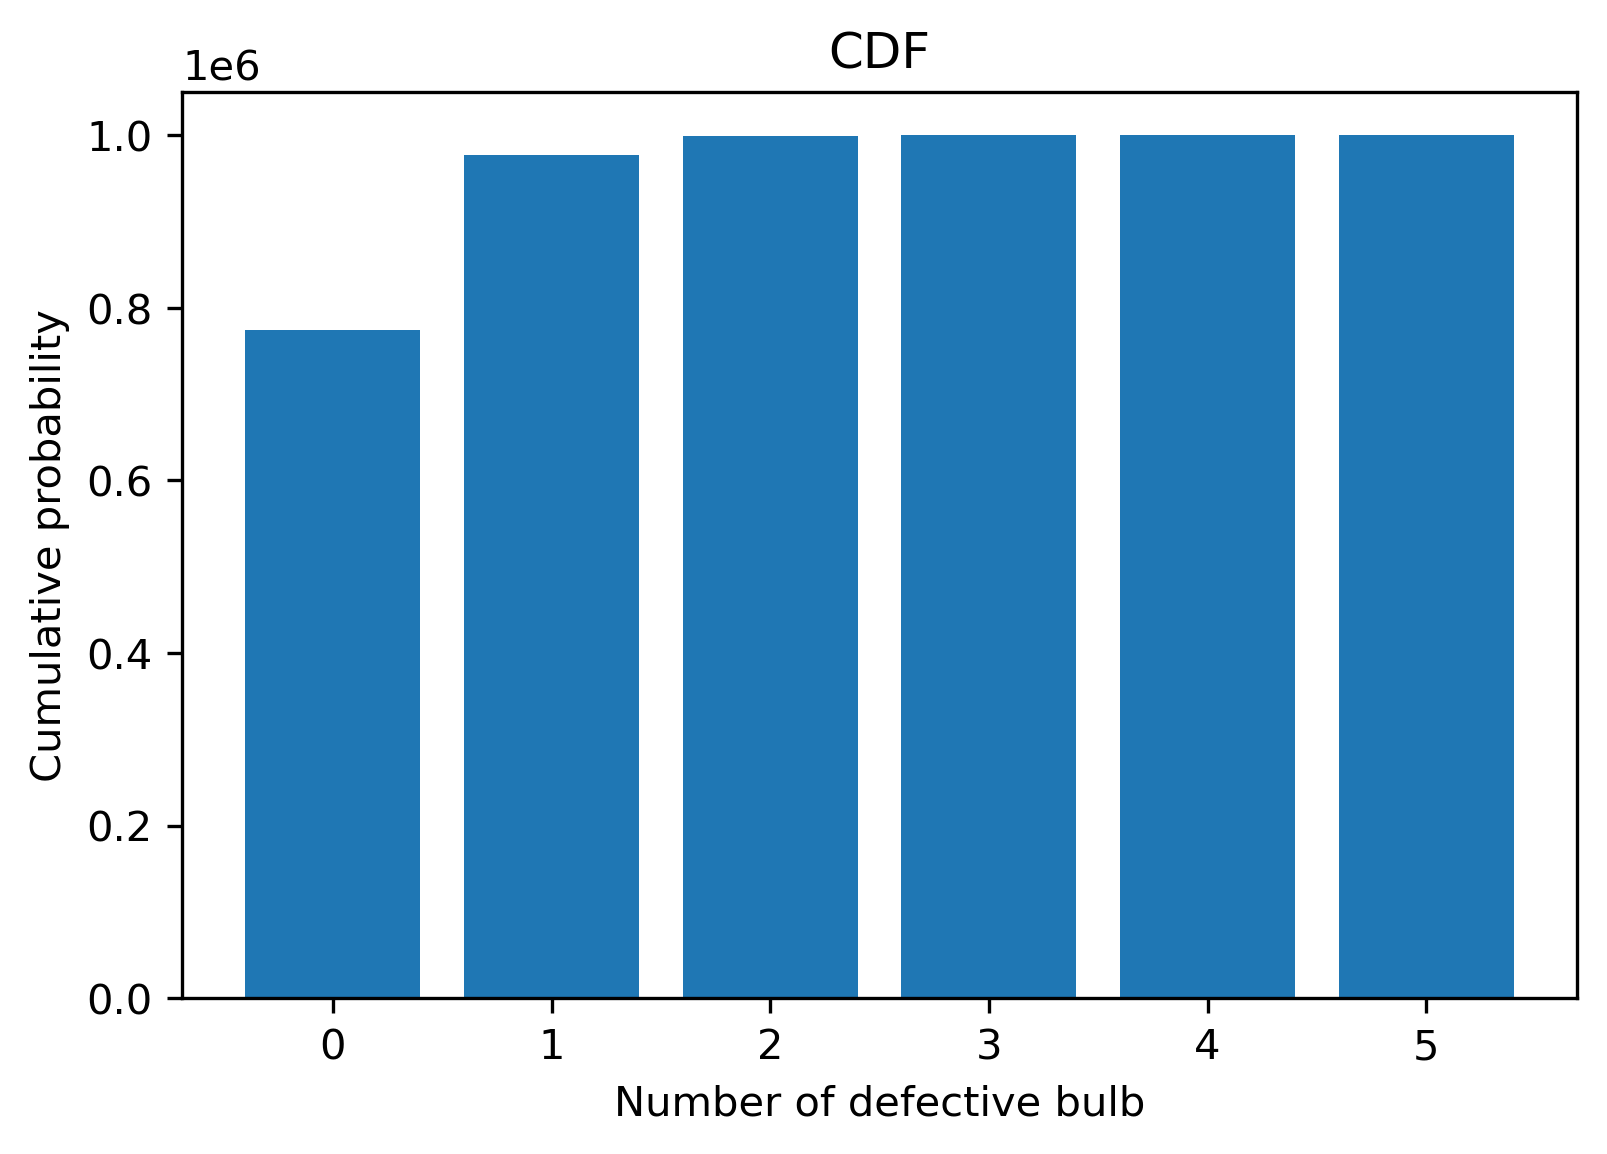
\includegraphics[width=9cm]{simulationCDF.png}
    \caption{simulated CDF plot}
\end{figure}
\begin{figure}[h!]
    \centering
    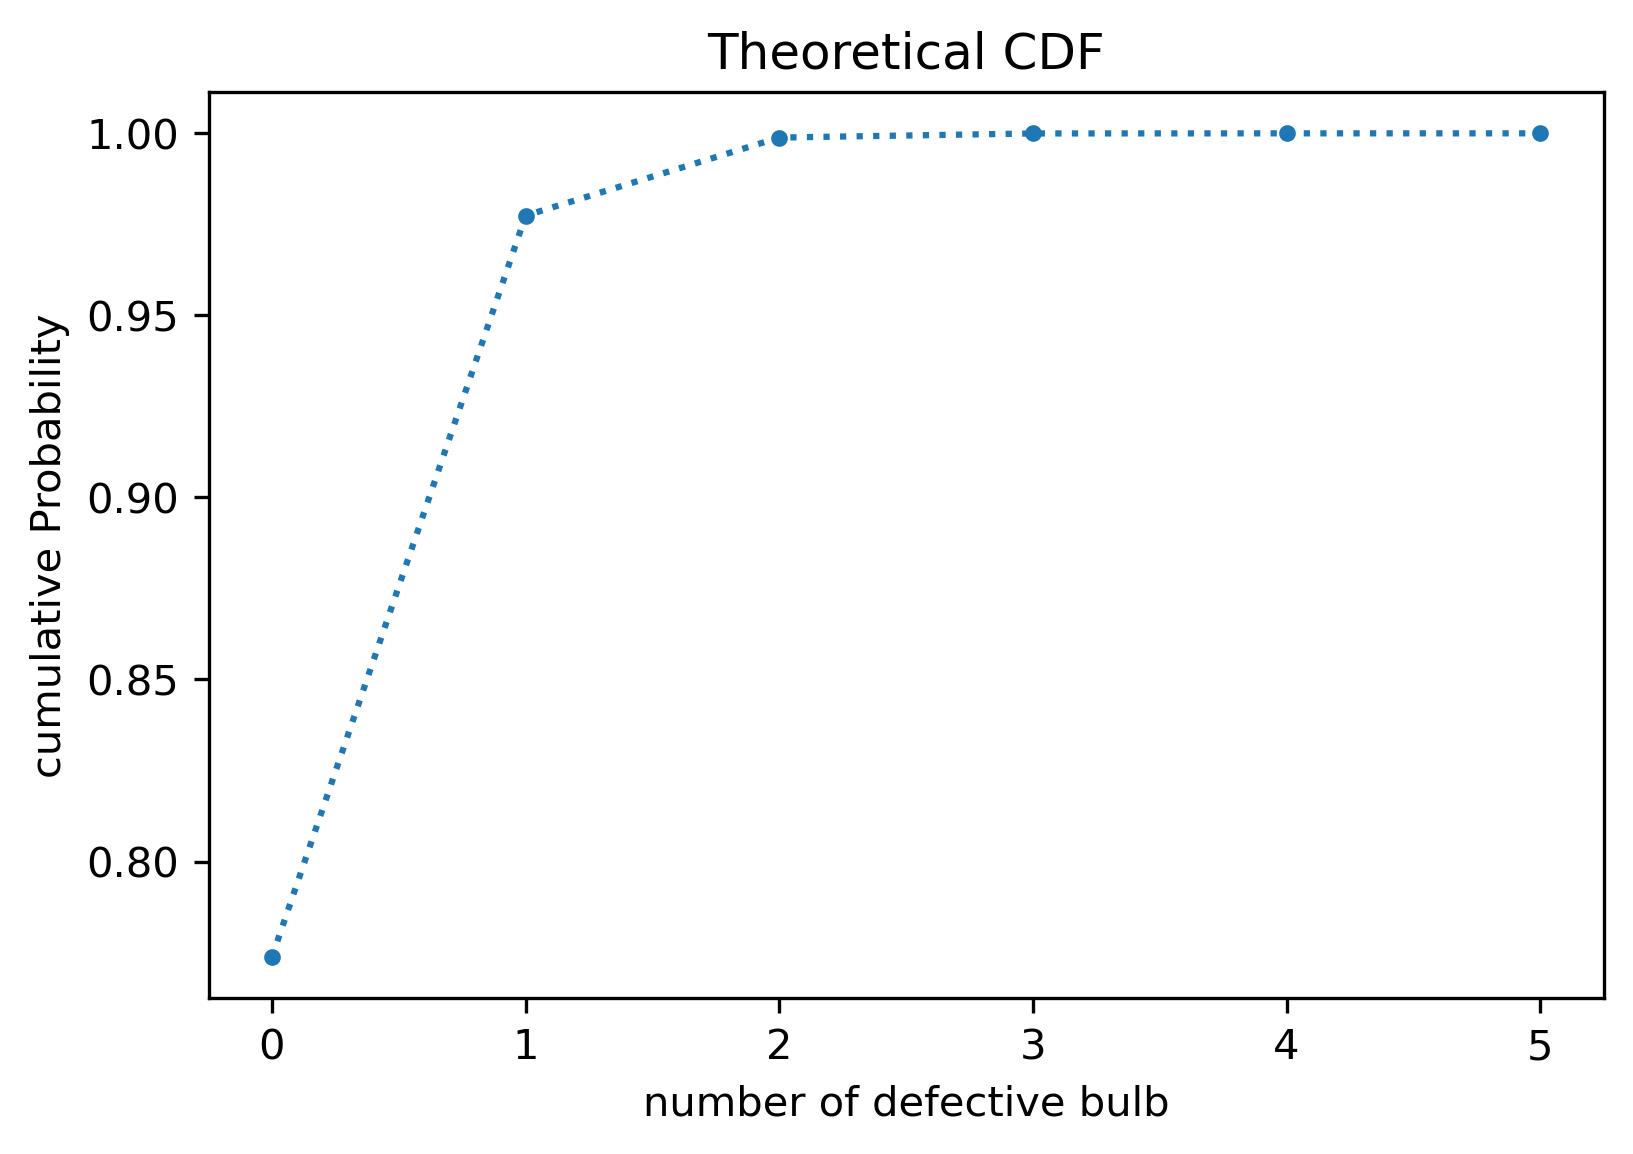
\includegraphics[width=9cm]{theoreticalCDF.png}
    \caption{theoretical CDF plot}
\end{figure}
\begin{figure}[h!]
    \centering
    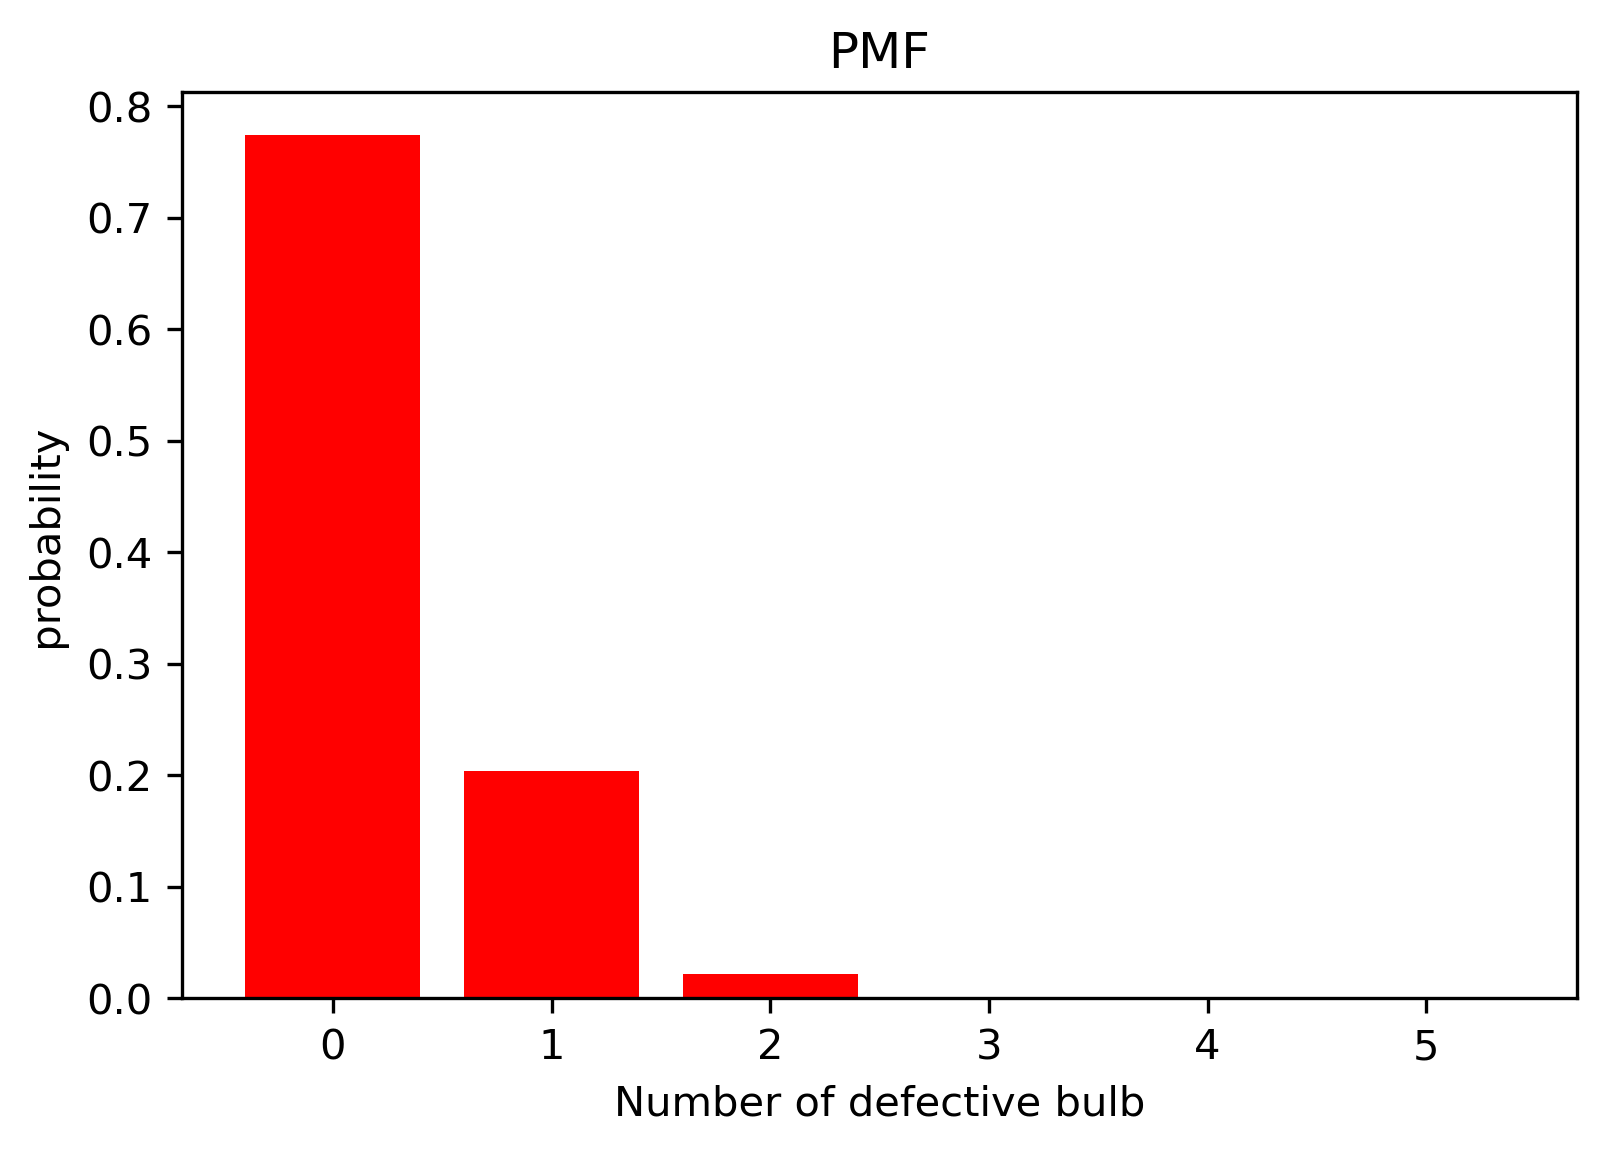
\includegraphics[width=9cm]{simulationPMF.png}
    \caption{simulated PMF plot}
\end{figure}
\begin{figure}[h!]
    \centering
    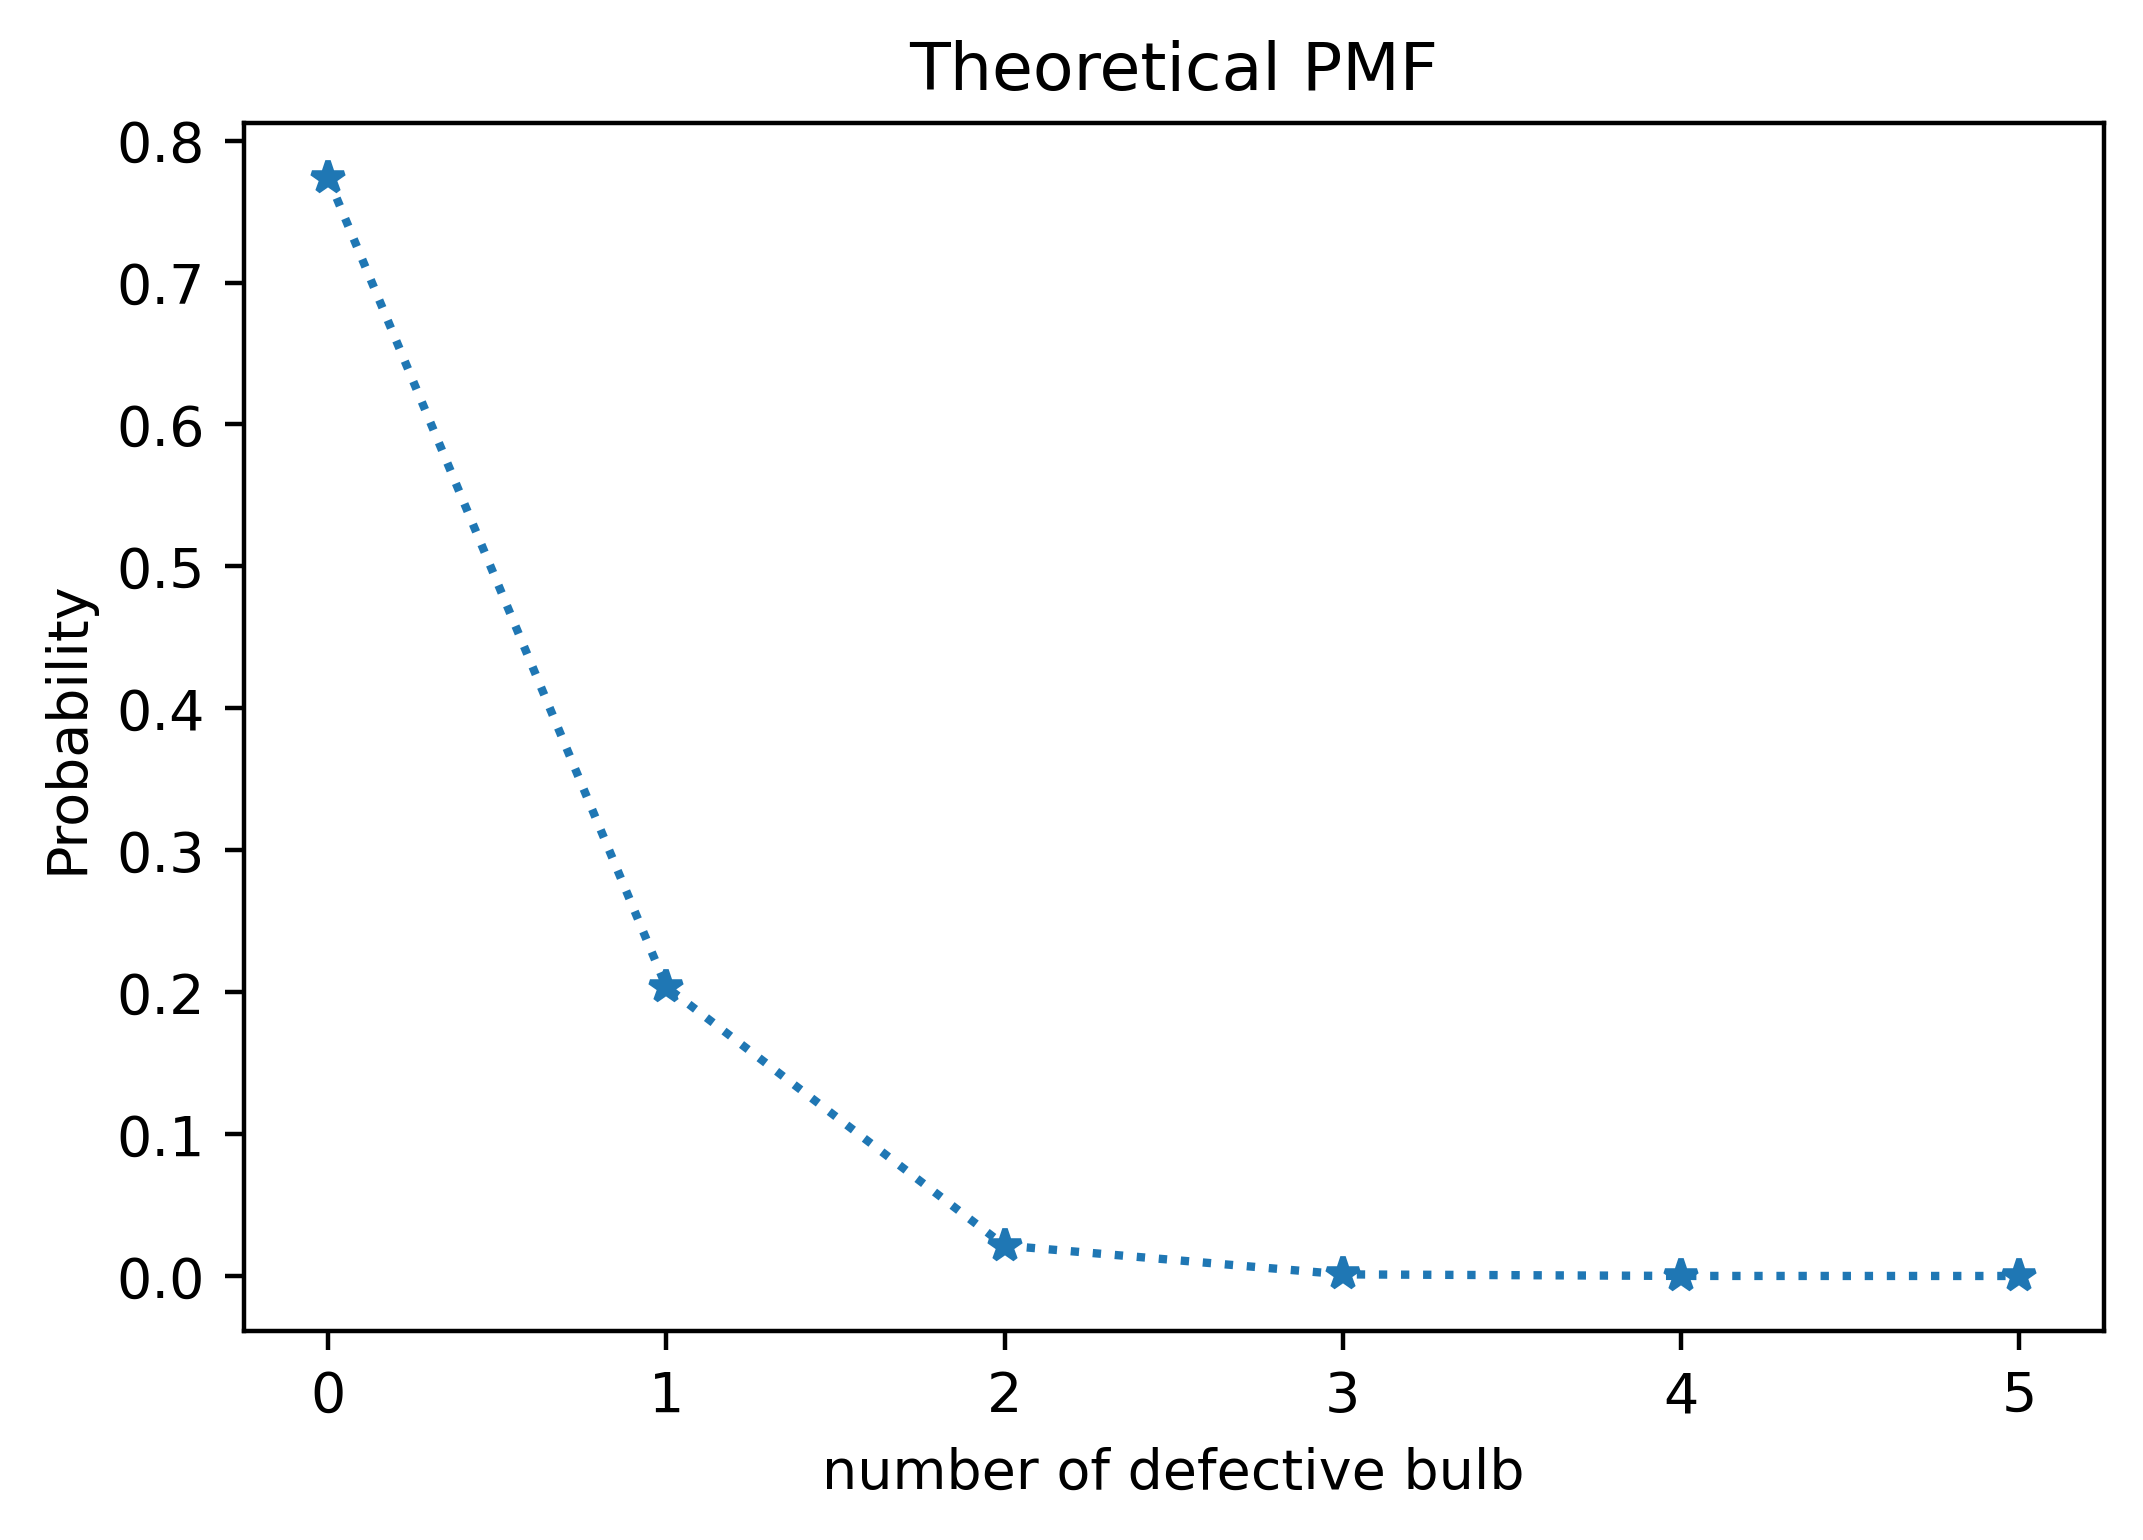
\includegraphics[width=9cm]{theoreticalPMF.png}
    \caption{theoretical PMF plot }
\end{figure}




\end{document}
